\documentclass{article}

\usepackage{fancyhdr}
\usepackage{extramarks}
\usepackage{amsmath}
\usepackage{amsthm}
\usepackage{amsfonts}
\usepackage{tikz}
\usepackage[plain]{algorithm}
\usepackage{algpseudocode}
\usepackage{graphicx}
\usetikzlibrary{automata,positioning}
\usepackage{pdfpages}

%
% Basic Document Settings
%

\topmargin=-0.45in
\evensidemargin=0in
\oddsidemargin=0in
\textwidth=6.5in
\textheight=9.0in
\headsep=0.25in

\linespread{1.1}

\pagestyle{fancy}
\lhead{\hmwkAuthorName}
\chead{\hmwkClass\ (\hmwkClassInstructor\ \hmwkClassTime): \hmwkTitle}
\rhead{\firstxmark}
\lfoot{\lastxmark}
\cfoot{\thepage}

\renewcommand\headrulewidth{0.4pt}
\renewcommand\footrulewidth{0.4pt}

\setlength\parindent{0pt}

%
% Create Problem Sections
%

\newcommand{\enterProblemHeader}[1]{
    \nobreak\extramarks{}{Problem \arabic{#1} continued on next page\ldots}\nobreak{}
    \nobreak\extramarks{Problem \arabic{#1} (continued)}{Problem \arabic{#1} continued on next page\ldots}\nobreak{}
}

\newcommand{\exitProblemHeader}[1]{
    \nobreak\extramarks{Problem \arabic{#1} (continued)}{Problem \arabic{#1} continued on next page\ldots}\nobreak{}
    \stepcounter{#1}
    \nobreak\extramarks{Problem \arabic{#1}}{}\nobreak{}
}

\setcounter{secnumdepth}{0}
\newcounter{partCounter}
\newcounter{homeworkProblemCounter}
\setcounter{homeworkProblemCounter}{1}
\nobreak\extramarks{Problem \arabic{homeworkProblemCounter}}{}\nobreak{}

%
% Homework Problem Environment
%
% This environment takes an optional argument. When given, it will adjust the
% problem counter. This is useful for when the problems given for your
% assignment aren't sequential. See the last 3 problems of this template for an
% example.
%
\newenvironment{homeworkProblem}[1][-1]{
    \ifnum#1>0
        \setcounter{homeworkProblemCounter}{#1}
    \fi
    \section{Problem \arabic{homeworkProblemCounter}}
    \setcounter{partCounter}{1}
    \enterProblemHeader{homeworkProblemCounter}
}{
    \exitProblemHeader{homeworkProblemCounter}
}

%
% Homework Details
%   - Title
%   - Due date
%   - Class
%   - Section/Time
%   - Instructor
%   - Author
%

\newcommand{\hmwkTitle}{Homework\ \#6}
\newcommand{\hmwkDueDate}{October 27, 2019}
\newcommand{\hmwkClass}{CMSE 820}
\newcommand{\hmwkClassTime}{}
\newcommand{\hmwkClassInstructor}{Professor Yuying Xie}
\newcommand{\hmwkAuthorName}{\textbf{Boyao Zhu}}

%
% Title Page
%

\title{
    \vspace{2in}
    \textmd{\textbf{\hmwkClass:\ \hmwkTitle}}\\
    \normalsize\vspace{0.1in}\small{Due\ on\ \hmwkDueDate\ at 11:59pm}\\
    \vspace{0.1in}\large{\textit{\hmwkClassInstructor\ \hmwkClassTime}}
    \vspace{3in}
}

\author{\hmwkAuthorName}
\date{}

\renewcommand{\part}[1]{\textbf{\large Part \Alph{partCounter}}\stepcounter{partCounter}\\}

%
% Various Helper Commands
%

% Useful for algorithms
\newcommand{\alg}[1]{\textsc{\bfseries \footnotesize #1}}

% For derivatives
\newcommand{\deriv}[1]{\frac{\mathrm{d}}{\mathrm{d}x} (#1)}

% For partial derivatives
\newcommand{\pderiv}[2]{\frac{\partial}{\partial #1} (#2)}

% Integral dx
\newcommand{\dx}{\mathrm{d}x}

% Alias for the Solution section header
\newcommand{\solution}{\textbf{\large Solution}}

% Probability commands: Expectation, Variance, Covariance, Bias
\newcommand{\E}{\mathrm{E}}
\newcommand{\Var}{\mathrm{Var}}
\newcommand{\Cov}{\mathrm{Cov}}
\newcommand{\Bias}{\mathrm{Bias}}

\begin{document}

\maketitle

\pagebreak

\begin{homeworkProblem}
\textbf{Solution}\\
\textbf{a. Encode training data}\\
We can use \(\phi\) to map the original data matrix to a data matrix \(\Phi(X)\) in the feature space, and perform dual PCA on the matrix \(\Phi^T\Phi\), i.e.,
\[
\Phi^T\Phi = V(\Sigma^2)V^T
\]
where \(\Phi=U\Sigma V^T\) is the compact SVD of \(\Phi\).  The first \(d\) principal components \(Y\in\mathbb{R}^{d\times n}\) are given by
\[
Y = \Sigma_d V_d^T
\]
where \(\Sigma_d\in\mathbb{R}^{d\times d} \text{ and } V_d\in \mathbb{R}^{n\times d}\) are truncated from \(\Sigma\) and \(V\), respectively.\\
\\
\textbf{b. Reconstruct training data}\\
The first \(d\) principal component eigenvectors are given by 
\[
U_d = \Phi V_d(\Sigma_d^{-1})
\]
The training data can be reconstructed in the feature space as 
\[
\tilde{\Phi}(X) = U_d Y = \Phi V_d(\Sigma_d^{-1})Y
\]

\textbf{c. Encode testing example}\\
\[
y^{\ast}=U_d^T\phi(x^{\ast}) = [\Phi V_d (\Sigma_d^{-1}]^T\phi(x^{\ast})
\]

\textbf{d. Reconstruct test example}\\
\[
\tilde{\phi}(x^{\ast}) = U_d y^{\ast} = \Phi V_d(\Sigma_d^{-1})y^{\ast}
\]

\end{homeworkProblem}


\begin{homeworkProblem}
The Algorithm was attached  in the following page, developed by Python.
\end{homeworkProblem}



\begin{homeworkProblem}
The results were attached in the following page followed by \(\textbf{Problem 2}\)
\end{homeworkProblem}


\begin{homeworkProblem}
The results were attached in the following page followed by \(\textbf{Problem 3}\)
\end{homeworkProblem}


\begin{homeworkProblem}
\textbf{1.} Show that \(K\succeq\) 0 if and only if its eigenvalues are all nonnegative.\\
\textbf{proof} Since \(K\) is symmetric and hence normal, there exists an orthogonal matrix \(Q\) ad a diagonal matrix \(\Lambda\) such that \(K=Q\)\(\Lambda\)\(Q^T\).
\[
\begin{split}
& K\succeq0 \\
\Longleftrightarrow\quad & \forall v\in \mathbb{R}^n, v^TKv=v^TQ\Lambda Q^Tv = (Q^Tv)^T\Lambda(Q^Tv)\geq 0\\
\Longleftrightarrow\quad & \Lambda\succeq0\\
\Longleftrightarrow\quad & \text{All eigenvalue of} K \text{are nonnegative.}
\end{split}
\]

\textbf{2.} Show that \(d_{ij}=K_{ii}+K_{jj}-2K_{ij}\) is a squared distance function, i.e., there exists vectors \(u_i, u_j\in\mathbb{R}^n \text{ for } 1\leq i,j\leq n\text{ such that }d_{ij}=\lVert u_i-u_j\rVert^2.\) \\
\textbf{proof} Let \(K=Q\Lambda Q^T\) be the eigenvalue decomposition of \(K\).  Define \(U = \Lambda^{\frac{1}{2}}Q^T\).  In particular, \(K=U^TU\), i.e., \(\forall i,j, K_{ij}=u_i^Tu_j \text{ where } u_i \text{ and }u_j \text{ are the } i\text{-th and the } j\text{-th columns of }U\), respectively.
\[
d_{ij}=u_i^Tu_i+u_j^Tu_j-2u_i^Tu_j = (u_i-u_j)^T(u_i-u_j) = \lVert u_i - u_j \rVert^2
\] 
 Thus d is a square distance function.\\
 
 \textbf{3.} Show that \(A+B\succeq0 \text{ and } A\circ B\succeq0\) (Hadamard product).  \\
 \textbf{proof} 
\[
\forall v\in\mathbb{R}^n, v^T(A+B)v = v^TAv+v^TBv\geq0 \Longrightarrow A+B\succeq0.
\]
 Let the eigenvalue decompositions of \(A\) and \(B\) be \(A=U\Lambda U^T=\sum_i\lambda_iu_iu_i^T\) and \(B = V\Gamma V^T=\sum_i \gamma_iv_iv_i^T\).
 \[
 A\circ B = \underset{i,j}{\Huge{\sum}}\lambda_i\gamma_j(u_iu_i^T)\circ(v_jv_j^T) = \underset{i,j}{\Huge{\sum}}\lambda_i\gamma_j(u_i\circ v_j)(u_i\circ v_j)^T
 \]
 Note that \(\forall x\in\mathbb{R}^T, x^T(u_i\circ v_j)(u_i\circ v_j)^T x = ((u_i\circ v_j)^Tx)^T((u_i\circ v_j)^Tx)\geq0, \text{ so }\forall i,j, (u_i\circ v_j)(u_i\circ v_j)^T\succeq0.\)  It follows that the nonnegative sum \(A\circ B\) of positive semi-definite matrices is also positive semi-definite.\\
 
 \textbf{4.} Show that the eigen values of \(AB\) are all positive given \(A, B\)  are symmetric positive definite matrix with the  same dimension.\\
 \textbf{proof} Let \(v\) be an arbitrary eigenvector of \(AB\) corresponding to the eigenvalues \(\lambda\), i.e., \(ABv=\lambda v\).  Assume \(A\succ0\) and \(B\succ0\).
 \[
 ABv = AB^{\frac{1}{2}}B^{\frac{1}{2}}v = \lambda B^{-\frac{1}{2}}B^{\frac{1}{2}}v \Longrightarrow (B^{\frac{1}{2}}AB^{\frac{1}{2}})(B^{\frac{1}{2}}v)=\lambda(B^{\frac{1}{2}}v).
 \]
 That is, an eigenvalue of \(AB\) must be eigenvalue of \(B^{\frac{1}{2}}AB^{\frac{1}{2}}\).  Note that \(\forall x\in\mathbb{R}^n, x^TB^{\frac{1}{2}}AB^{\frac{1}{2}}x= (B^{\frac{1}{2}}x)^TA(B^{\frac{1}{2}}x)>0\).  So all eigenvalues of \(AB\) are positive.\\
 
 \textbf{5.} If \(A\succeq0\) and \(c\geq 0\), then \(cA\succeq0\)\\
 \textbf{proof} 
 \[
 \forall x\in\mathbb{R}^n, x^TcAx=cx^TAx\geq0\Longrightarrow cA\succeq0.
 \]
 \\
 
 \textbf{6.} If \(A\succeq0\) and \(C\) can be written as \(C=\{t_{[i]}A_{ij}t_{[j]}\}\) for \(\forall t\in\mathbb{R}^n\), then \(C\succeq0\).\\
 \[
 \forall x\in\mathbb{R}^n, \underset{i,j}{\Huge{\sum}}x_ix_jC_{ij}=\underset{i,j}{\Huge{\sum}}(x_it_{[i]})A_{ij}(x_jt_{[j]})\geq 0 \Longrightarrow C\succeq 0.
 \]
 \\
 
 
 \textbf{7.} Show that the Hadamard integral power \(A^{\circ p}= \{A_{ij}^p\}\) and \(p\in\mathbb{N}\) and Hadamard exponential exp(\(\circ A\)) = \(\{\text{exp}(A_{ij})\}\) are p.s.d..\\
 \textbf{proof} By (3),
 \[
 A\succeq0\Longrightarrow A^{\circ2}=A\circ A\succeq 0
 \]
 By induction,
 \[
 \forall p\in\mathbb{N}, A^{\circ p}\succeq 0.  \quad\text{exp}(\circ A) = \Huge{\sum}_{p=0}^{\infty}\frac{A^{\circ p}}{p!}\succeq0.
 \]
Note that the finite sum \(S_n(A)=\Huge{\sum}_{p=0}^n\frac{A^{\circ p}}{p!}\) is p.s.d., and \(\{S_n\}\) converges uniformly to exp(\(\circ A\)).

\end{homeworkProblem} 



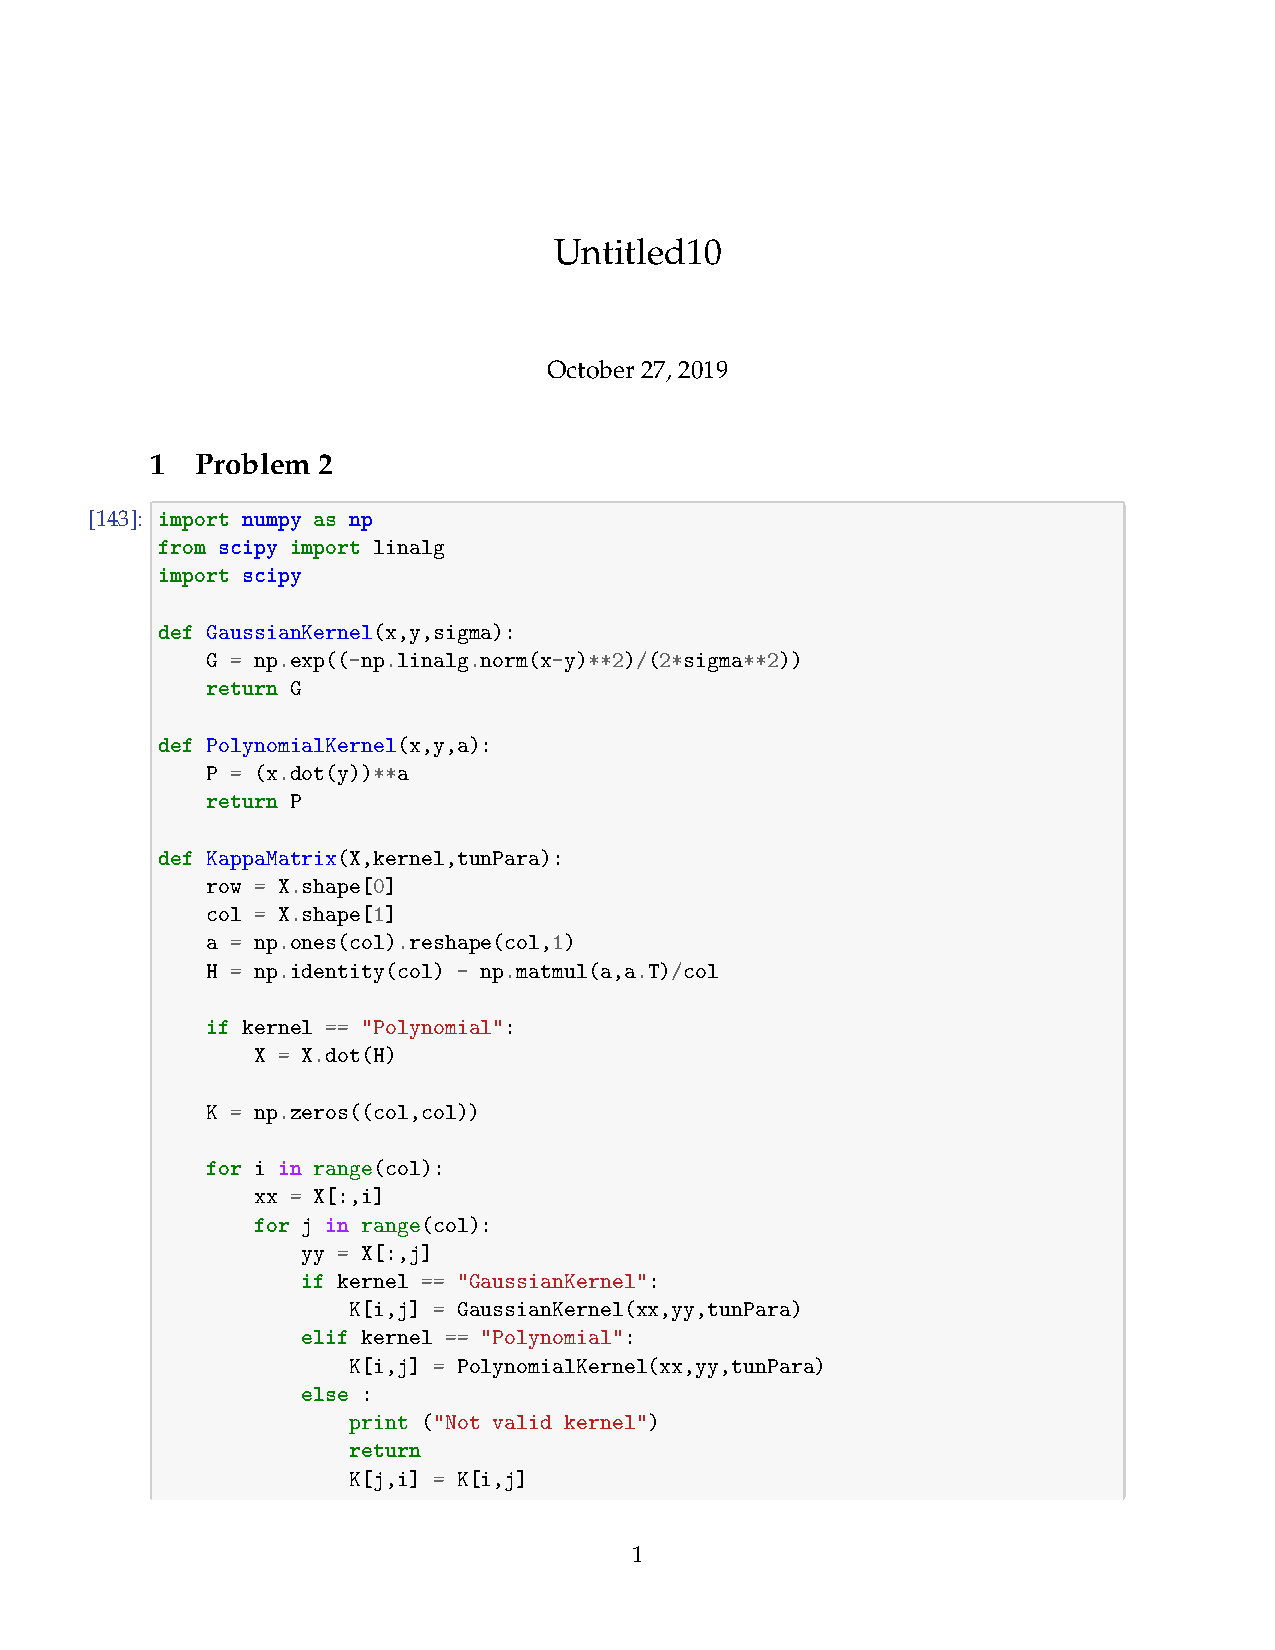
\includepdf[page={-}]{Untitled10.pdf}









































\end{document}